\documentclass[conference]{./IEEEtran}

%\usepackage{ulem} 
%% \usepackage{subfigure}
%% \usepackage{comment}
%% \usepackage{graphicx}
%% \usepackage{algorithm}
%% \floatname{algorithm}{Procedure}
%% \usepackage{multirow}
%% \usepackage{makeidx}
%% \usepackage{amsmath}
%% \usepackage{amssymb}
%% \usepackage{epsf}
%% \usepackage{pstricks}
%% \usepackage{pst-grad}
%% \usepackage{placeins}
%% \usepackage{url}
%% \usepackage{epsfig}
%% \usepackage{multirow}
%% \usepackage{pifont}
%% \usepackage{graphics}
%% \usepackage{color}
%% \usepackage{epsf}
%% \usepackage{mathcomp}
%% \usepackage{colordvi}
%% \usepackage{epsfig}
%% \usepackage{fancyhdr}
%% \usepackage{wasysym}
%% \usepackage{longtable}
%% \usepackage{afterpage}
%% \usepackage{colordvi}
%% \usepackage{latexsym}
%% \usepackage{float}
%% \usepackage{alphalph}
%% \usepackage{epic,eepic}
%% \usepackage{authblk}
%% \usepackage{algpseudocode}
%% \usepackage{mathptmx}



%% \newtheorem{definition}{Definition}
%% \newtheorem{example}{Example}
%% \newtheorem{note}{Note}
%% \newtheorem{operation}{Operation}
%% \newtheorem{axion}{Axion}
%% \newtheorem{remark}{Remark}
%% \newtheorem{lemma}{Lemma}
%% \newtheorem{theorem}{Theorem}

\ifCLASSINFOpdf
  % \usepackage[pdftex]{graphicx}
  % declare the path(s) where your graphic files are
  % \graphicspath{{../pdf/}{../jpeg/}}
  % and their extensions so you won't have to specify these with
  % every instance of \includegraphics
  % \DeclareGraphicsExtensions{.pdf,.jpeg,.png}
\else
  % or other class option (dvipsone, dvipdf, if not using dvips). graphicx
  % will default to the driver specified in the system graphics.cfg if no
  % driver is specified.
  % \usepackage[dvips]{graphicx}
  % declare the path(s) where your graphic files are
  % \graphicspath{{../eps/}}
  % and their extensions so you won't have to specify these with
  % every instance of \includegraphics
  % \DeclareGraphicsExtensions{.eps}
\fi

\hyphenation{op-tical net-works semi-conduc-tor}
\begin{document}

\title{Adaptive Display Scheme over Real-time Multimedia Communication on Mobile Devices}

%for single author (just remove % characters)
%%\date{}
%% \special{papersize=8.5in,11in}
%% \setlength{\pdfpageheight}{\paperheight}
%% \setlength{\pdfpagewidth}{\paperwidth}

%% \conferenceinfo{Submission to SoCC '14}{October, 2014, Seattle, WA, USA} 
%% \copyrightyear{2014} 
%% \copyrightdata{978-1-nnnn-nnnn-n/yy/mm} 
%% \doi{nnnnnnn.nnnnnnn}


\author{
  \IEEEauthorblockN{Mengbai Xiao}
  \IEEEauthorblockA{
    mxiao3@gmu.edu\\
    Department of Computer Science\\
    George Mason University}
    \and
  \IEEEauthorblockN{Songqing Chen}
  \IEEEauthorblockA{
    sqchen@gmu.edu\\ check the email\\
    Department of Computer Science\\
    George Mason University}
}

%% \author
%%     {
%%       \IEEEauthorblockN{Mengbai Xiao}
%%     }
%% \author{\IEEEauthorblockN{Michael Shell}
%% \IEEEauthorblockA{School of Electrical and\\Computer Engineering\\
%% Georgia Institute of Technology\\
%% Atlanta, Georgia 30332--0250\\
%% Email: http://www.michaelshell.org/contact.html}
%% \and
%% \IEEEauthorblockN{Homer Simpson}
%% \IEEEauthorblockA{Twentieth Century Fox\\
%% Springfield, USA\\
%% Email: homer@thesimpsons.com}
%% \and
%% \IEEEauthorblockN{James Kirk\\ and Montgomery Scott}
%% \IEEEauthorblockA{Starfleet Academy\\
%% San Francisco, California 96678-2391\\
%% Telephone: (800) 555--1212\\
%% Fax: (888) 555--1212}}


\maketitle


%% \author[1]{Mengbai Xiao}
%% \author[2]{Ming Zhang}
%% \author[1]{Songqing Chen}
%% \affil[1]{\{mxiao3,sqchen\}@gmu.edu, Department of Computer Science, George Mason University}
%% \affil[2]{ming.zhang@emc.edu, Advanced Software Division, EMC}
%% \renewcommand\Authands{ and }
%% \maketitle 



%\thispagestyle{empty}

%\sloppy
%------------------------------------------------------------------------------

\begin{abstract}

On a mobile device, the display subsystem ususally consumes 30\%-60\%
of the total battery power.  As such, a few designs have aimed to
reduce the display power consumption in mobile video streaming.  The
basic idea is to dim the backlight level while properly compensating
the pixel luminance to maintain image fidelity.  The luminance
compensation and proper luminance calculation are computation
intensive and demand per-frame luminance information. Thus, existing
schemes only target video-on-demand where the luminance information of
each frame is available in advance. In addition, they demand
additional computing resource support. Otherwise, if the computation
is conducted on the mobile device, the computing
overhead can easily offset the power saving.  In this work, we set to
investigate power saving for video calls on mobile devices.  Different
from video-on-demand, the real-time video calls are highly delay
sensitive and the frame luminance information is not known in
advance. Moreover, video calls often involve multiple
streaming sources from multiple ($\ge$2) participants, making it more
difficult.  Because there are fewer background changes and a often
slower frame rate in video calls, we design a greedy display power
saving scheme, called LCD-GDP, by utilizing the commonly available GPU on mobile
devices without demanding additional support.  Our design is
implemented on WebRTC, a popular real-time web browser based video
call standard.  Experiments show that our scheme can save upto 40\%
power consumption in video calls.

%% Power saving is a significant issue at the mobile platform. Various
%% techniques were proposed to extend the playback time of the
%% videos. Backlight scaling is one of them and target the display
%% subsystem. However, the multimedia content need to be delivered in a
%% timely manner in the real-time communication. This raises challenges
%% towards the existing backlight scaling technique. The backlight
%% scaling technique is composed of computation intensive tasks,
%% including the luminance histogram generation and the pixels
%% luminance compensation on every frame. Multiple streaming sources in
%% the video conference make this problem more difficult. Moreover,
%% global luminance information is necessary for finding the optimal
%% backlight levels across the streaming. This is clearly impossible in
%% the real-time case. In this paper, we propose a greedy algorithm
%% determining the backlight level of current frame only from the last
%% one. We also take advantage of the GPU to relive the burden of the
%% CPU on compensating the luminance of pixels. We integrate our
%% prototype in the AppRTC, an Android app based on WebRTC, and find
%% that our scheme can save up to 39.8\% energy during one
%% communication session.
\end{abstract}


\section{Introduction}


With the ever-improving network and mobility support, recently,
real-time communication software, being standalone or combined with
social media, have also found their way on mobile devices.  Being able
to support video calls while entirely free or at least cheaper than
the traditional voice communications, these software, such as
Skype~\cite{skype}, QQ~\cite{qq}, Apple's Facetime~\cite{facetime},
and Google WebRTC~\cite{webrtcproject}, are quickly gaining popularity
among common mobile users.


However, the limited battery power supply remains as the Archille's
heels of mobile devices while real-time video communications are very
power-hungry. Compared to the video streaming, real-time video calls
are more demanding. In the real-time video communication, such as the
video conferencing, the video contents are generated on the fly from
multiple sources. Even for the one-to-one video call, double frames
are generated other than the common video streaming. Thus, efficiently
reducing the power consumption for video calls on mobile devices is
imperative.


Previously, since the display subsystem on a mobile device often
consumes about 38\% to 68\% of the total energy during video
streaming~\cite{AG10}, a few schemes have been designed to reduce the
power consumption of the display. For a Liquid-Crystal Displays (LCD)
display, the dominant power consumption is by the backlight
intensity. Thus to reduce the power consumption, it is desirable to
dim the backlight as much as possible while enhancing the luminance of
the pixels to comprensate the quality degradation due to backlight
dimming.  In this way, the modified images on the screen can maintain
image fidelity to the human's eyes. Such a technique is called
backlight scaling.

In detail, the backlight scaling technique often consists of three
stages, i.e., 1) the histogram generation stage, 2) the backlight
levels determination stage, 3) the pixel compensation stage. The first
stage and the last stage are both computation intensive. Therefore,
some previous design either ignore the luminance
compensation~\cite{HLH11}, leading to significant quality degradation
and user experience unsatisfaction, or demand additional computing
resources for compensation~\cite{LHH14}, making the scheme
non-practical for mobile devices.  In the second stage, some previous
research applies the dynamic programming to find the globally optimal
backlight levels without violating the hardware and user experience
constraints. Thus, the video frames must be available in advance.
However, for real-time video calls, this is impossible because the
video content is generated on the fly.  Furthermore, being higly
sensitive to delay, real-time video calls cannot tolerate the delay
that may be caused by the dynamic programming. In addition, by often
supporting multiple participants and thus receiving data from multiple
sources simultaneously, the backlight scaling technique cannot be
directly used for video calls.

In this paper, we set to explore the display power saving for video
calls on mobile devices. Since there are often less background changes
and slower frame rate in practical video calls, we propose a greedy
display power saving scheme, called {\it LCD-GDP}.  Similar to the dynamic programming
approach for video streaming, there are same constraints that our
greedy algorithm must conform to. The {\it first} is that the backlight
variations between neighboring frames must be limited. Otherwise the flickering effect is expected
in the user experience~\cite{}. {\bf add reference here} The {\it second} is that the backlight should not be
scaled down too much to cause image distortion~\cite{}. {\bf add
  reference}  The {\em third} is that the
backlight cannot be adjusted too frequently because the hardware needs some time
to respond~\cite{}. {\bf add reference}


To avoid processing the same frame repeatedly, in LCD-GDP, {\it first}, we migrate
the histogram generation to the sender side for video calls. We
put the luminance information inside each frame without building an
additional channel. Also duplicated information is hidden for the
possible loss during the video encoding/decoding and the network
transmission.

{\it Second}, since GPU is commonly equipped in the mobile devices, we
take advantage of GPU to offload some tasks from the
CPU. For the purpose of rendering the received frames in a timely
manner, we use the OpenGL ES 2.0 shaders to perform the pixel
enhancement.  Moreover, the power savings will not be offset by
enabling GPU since GPU is widely used in the video conferencing for
composing frames together and then rendering them.

To evaluate the performance of our design, we implement LCD-GDP into
WebRTC and run experiments on a tablet and a smartphone. Experimental
results show that {\bf by using the LCD-GDP, the metric of frames per
  second doesn't decrease obviously and only additional tens of
  milliseconds are found in latency. Upto $33.2\%$ power consumption
  can be saved on average due to the brightness of the
  environment. }

This paper is organized as follows. We describe some background
information for both backlight scaling and WebRTC 
%is introduced and some related work is reviewed 
in Section \ref{sec:background}. We present
our design in Section \ref{sec:design} and the implementation details
in Section \ref{sec:implementation}. We discuss
the evaluation in Section \ref{sec:evaluation} and conclude our work
in Section \ref{sec:conclusion}.


%% old representation
\if 0
The great success of the real-time communication has been witnessed in
the last decade. The popular software, like Skype, QQ and Apple's
Facetime, make the real-time communication as a cheaper alternative to
the calls. Nowadays, with the emerging mobile market, these
applications were migrated to the mobile platform as well. However,
like the other mobile applications, the power issue is hindering the
deployment of real-time communication on the mobile
devices. Especially in the real-time communication app, several
power-hungry modules, like wireless network, camera and etc. So
maximizing the power savings is desired and attractive in the
real-time communication.


According to the previous research ~\cite{AG10}, about 38\% to 68\% of the
total energy is consumed by the display subsystem during the video
playback, and this portion is growing on the new generation of
devices, which are equipped with more powerful GPUs and more
large-sized display panels. We also expected the average power
consumption during the real-time communication will be cut down if the
display subsystem is optimized. One existing technique, named
backlight scaling, can be used to reduce the energy consumption of
Liquid-Crystal Displays (LCD). The power consumption of LCD is
dominated by the backlight intensity, so this technique tries to dim
the backlight as much as possible while enhancing the luminance of the
pixels, which are rendered on the screen, at the same time. In this
way, the modified images on the screen are perceived as the original
ones by the human eye.  


In this paper, we explored the possibility of deploying the backlight
scaling technique with the real-time communication. The backlight
scaling technique is composed of three stages. 1) Histogram generation
stage. 2) Backlight levels determination stage. 3) Pixels compensation
stage. The first stage and the last stage are both computation
intensive tasks when performing these operations on each frame. In the
second stage, previous research applies the dynamic programming to
find the globally optimal backlight levels without violating some
constraints. Not only is the extra CPU time required, but also the
backlight levels can be determined on-the-fly. All of these obstruct
the backlight scaling technique being applied in the real-time
communication.

In the real-time communication, like the video conferencing, the video
contents are generated from multiple sources. Even for the one-to-one
video call, double frames are generated other than the common Internet
streaming, like watching the movies. To avoid processing the same
frame repeatedly, we migrate the histogram generation stage to the
sender side. We put the luminance information inside each frame
without building an additional channel. Also duplicated information is
hidden for the possible loss during the video encoding/decoding and
the network transmission.

The dynamic programming algorithm is necessary in the common video
playback scenario since there are some constraints we have to conform
to. The backlight variations must be limited when the flickering
effect is not expected in the user experience. Also the backlight
should not be scaled down too much to cause the distortion. However,
the dynamic programming is not applicable in real-time communication
due to the dynamically generating video contents. Even if this
algorithm is partially applied, significant delays are introduced in
the sessions. Fortunately, in the real-time communication, we can risk
scaling the backlight levels in greedy manner because no scenes
switching are expected. 

When the GPU is commonly equipped in the mobile devices, we are able
to take advantage of this facility to offload some tasks from the
CPU. For the purpose of rendering the received frames in timely
manner, we use the OpenGL ES 2.0 shaders to perform the pixels
enhancement stage. Little delays are introduced in this way. Moreover,
the power savings won't be offset by enabling GPU since GPU is widely
used in the video conferencing for composing frames together and then
rendering them.

This paper is organized as follows: the background is introduced and
some related work is reviewed in Section \ref{sec:background}. We propose
our design in Section \ref{sec:design}. The details of implementation
are illustrated in Section \ref{sec:implementation}. Then we discuss
the evaluation in Section \ref{sec:evaluation} and conclude our work
in Section \ref{sec:conclusion}.
\fi


%% The real-time communication, as a considerably
%% cheaper alternative to the calls, makes QQ, Skype, Apple's
%% Facetime and etc. so popular all round the world. More attractively,
%% with the bandwidth growth of the Internet, the real-time communication
%% is always equipped with the video channel so that two ends can talk
%% face-to-face. Now the prosperity of mobile devices, including
%% smartphones, tablets and emerging wearable devices, offers another
%% available platform for the real-time communication. The real-time
%% communication is more desired on these portable devices, which can
%% benefit from the wireless networks everywhere. However, new challenges
%% to deliver video stream on the mobile devices have raised and one of
%% them is to maximize the power savings.


% stress the importance real-time communication on mobile devices
% This part is redundant, make it concise.
% Don't discuss the details of WebRTC. Only mention the general idea
% of Real-time communication.


%% On the other hand, Dynamic Adaptive Streaming over
%% HTTP(DASH) makes a salient example that how multimedia streaming is
%% delivered nowadays. WebRTC(Web Real-Time Communication), technique
%% that integrating real-time communication over HTTP, is standardized by
%% W3C and the IETF. Thus a cross-platform solution will be handy and the
%% growth of real-time communication on new platform is
%% expected.
%% As an advanced functionality, video call becomes an essential
%% component in many *communication applications/wechat, skype... check
%% in twin cloud paper*. The needs for unifying the interface is
%% increasingly desirable. The success of DATH *add name* hints people
%% the importance of HTTP in video/audio streaming scenarios. WebRTC as a
%% new API existing in HTML5 drops in developer's sight. Mainstream
%% browsers integrates the function into there production, i.e. Chrome,
%% Opera, Firefox. Developers can easily include video call in their page
%% via few lines of javascript code.


%% In this paper, we explored the possibility if an effective LCD
%% power-saving technique, named luminance compensation, can be applied
%% on the real-time communication services. There are three steps in this
%% technique. 1) Extract the luminance histrogram of the frames. 2)
%% Decide the backlight levels and do scaling when the frames are
%% rendered. 3) According to the backlight levels, enhance the luminance
%% component of the pixels. This technique has been successfully adopted
%% on some other streaming services, however, there are still 
%% several challenges in the real-time case:
%% \begin{itemize}
%%   \item
%%     {
%%       Unlike the other streaming services of predefined content, in
%%       real-time communication, there is no way to build a utility to
%%       extract and analyze the videos in the offline manner. The extraction
%%       process, which is computation intensive, has to be installed
%%       along with the services. 
%%     }
%%   \item
%%     {
%%       In a N-party communication, $N$ frames are rendered on one screen
%%       at the same time. $N$ times the input data makes the extraction
%%       operation even worse.
%%     }
%%   \item
%%     {
%%       To decide the backlights levels, a dynamic programming algorithm
%%       has been proposed. However, this handy soloution requires large
%%       buffer size to collect enough luminance information and then to
%%       reach the global optimal result. However, this is not practical
%%       in the real-time case.
%%     }
%% \end{itemize}

%% designed a system composed three components in the names of {\bf
%%   Scanning Module}, {\bf Adjustment Module} and {\bf Rendering
%%   Module}. These components are integrated into real-time
%% communication.


% conventional
%% On the other hand, people doesn't satisfy themselves with traditional
%% phone call, which make them only listen to their relatives. On
%% smartphone, installing communication applications becomes available
%% and people can also see the other end over one call. *not only on the
%% traditional PC*. Moreover, video call is much cheaper, sometimes even
%% free. In the future day, we can easily make video call over webRTC,
%% the unifying interface in browsers. Since both on the mobile and PC we
%% can access it via browsers. Even more, Google has been making effort
%% on packaging their implementation in Chrome as available for Android
%% App developers. So we can make such call via the simple thing.

%% The power-saving scheme for VoIP is few, since the most applications
%% are properties of company. Researchers is hard to figure out which
%% part is enable to save the energy. Also the old applications are
%% designed for PC client. The achievement is in the network layer,
%% adapting the transmission protocols to specific scenarios *I guess,
%% check it*. On the other hand, many effective energy effective schemes
%% were proposed for streaming on mobile platform, such as *give some
%% example, ref to our paper*. This motivate us to put these schemes in
%% the real-time multimedia case.

%% Thanks to Google, the Chromes is an open source project, in the nature
%% of things the WebRTC is part of it as libjingle*introduce to
%% libjingle*. More fortunately, the libjingle is able to be integrated
%% as 3rd library with Android applications. So the Android application
%% can take advantage of this aside web browsers.

%% Display is the most great part of mobile power consuming. As
%% LCD*introduce the LCD?*, one 
%% efficient way to save power is adjust the backlight with compensating
%% the pixels. there are works done on the local video case and online
%% streaming case. Usually the GPU is used to dynamically scan frames and
%% retrieve the highest pixels. we have some opportunities:
%% \begin{itemize}
%%   \item
%%     {
%%       % Challenge: Cooperation
%%       In the real-time case, or the p2p case, video is generated via
%%       clients. We don't need to passively accept the frame and parse
%%       frames until them are decoded. On the other hand, we can scan
%%       the frames before encoding when the stream is
%%       generated. How can we effectively do this? one challenge is how
%%       we pass the information to the other side. we
%%       don't need to open another data channel on this. put the max
%%       pixel at the corner.
%%       *We can also split the scanning process*
%%       we offload the DP part to the receiver.
%%     }
%%   \item
%%     {
%%       % Challenge: take advantage of the scenarios
%%       Also the real-time communication has its characteristics. The
%%       frames staying relative still. We can adjust the max liminance
%%       in greedy manner. More aggressively, we can adjust the frames
%%       in case of skipping some frames. 
%%     }
%%   \item
%%     {
%%       % Challenge: graphical composition
%%       The receiver is asked to compose frames received from several
%%       senders. 
%%     }
%%   \item
%%     {
%%       % The DP problem
%%       The DP is not optimal if the power-backlight is not linear
%%       relationship. But the Greedy is even more not optimal.

%%       In real-communication users is more likely to be tolerant. 
%%     }
%% \end{itemize}





%% \input{overview}

%% \section{System Design}
\label{sec:design}
%In this section, we present our design of LCD-GDP.

\subsection{System Components}
As we discussed before, the backlight scaling generally involves three
steps for 1) generating the luminance histogram, 2) determining the
proper backlight levels and 3) compensating the pixel luminance. In
our system, we decouple them into the following three independent
modules: the {\bf Scanning} module, the {\bf Adjustment} module, and
the {\bf Rendering} module. Next we present our new approaches in
these three modules, respectively. Figure~\ref{fig:design} illustrates
the organization and interaction of these three modules.

\begin{figure}[t]
  \centering
%  \label{fig:design}
  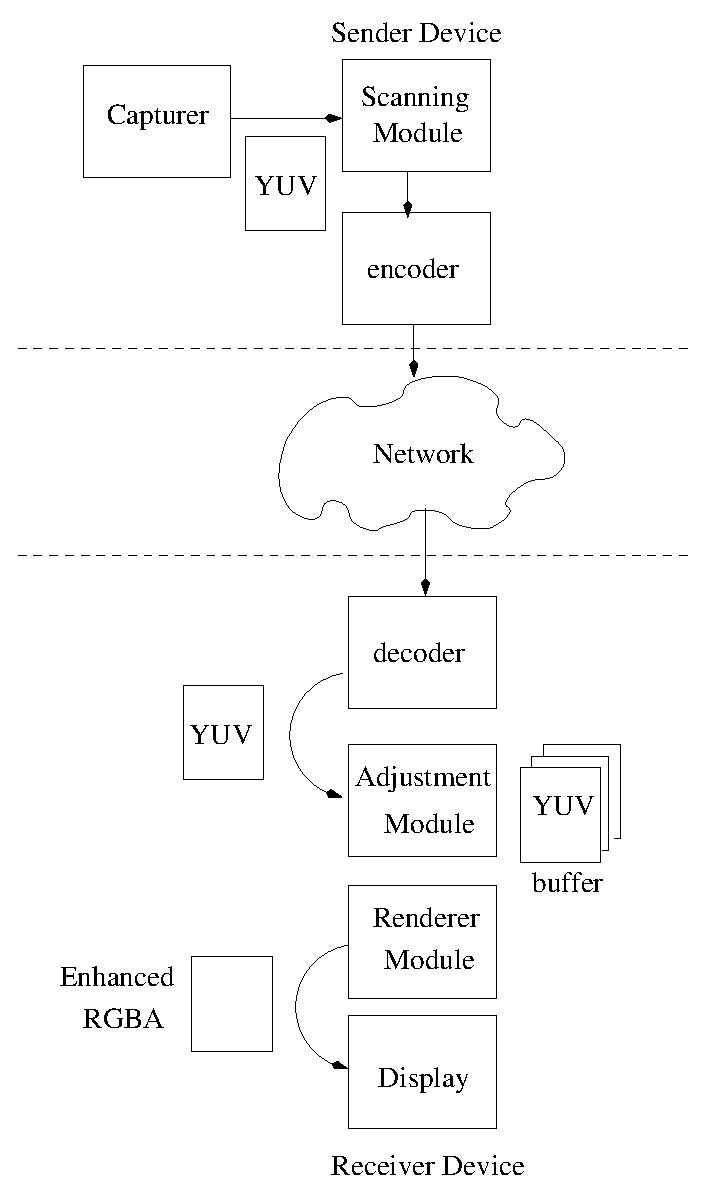
\includegraphics[width=.45\textwidth]{./figures/design.eps}
  \caption{LCD-GDP system architecture and major components}
\label{fig:design}
\vspace{-2em}
\end{figure}



\noindent{\bf Sender-Side Scanning and Piggybacking}:
The {\bf Scanning} module is the component to extract the pixel
luminance information. In the real-time communication, the frames are
generated by the capturer, which is usually a physical camera. There
is no way to access the whole video content in advance. So the
scanning module is necessary to generate the luminance histogram for
later determination stage and compensation stage. Other than the Video
On Demand (VOD), the RTC session involves $N \ge 2$ participants, and
the rendered image is composed by all received frames (including that
from the receiver itself). While it is natural to conduct the scanning
after receiving the image, in our design,  the scanning module is
installed at the sender side so that each generated frame will be
scanned only once. (Otherwise, every receiver needs to conduct the
scanning for the same image repetitively.)  However, this brings
another problem: how to transmit this luminance information to the
receivers if the scanning is done on the sender side. Building another
channel is possible, but it introduces additional overhead and extra
efforts must be made to synchronize the frames and the luminance
information. Either of them may not arrive the receiver on time.

To this end, we choose to encode this information with the frame data
for more efficiency on the luminance information transmission.  In our
scheme, the bottom corners are the best candidates. This position
either is covered by other frames, or is negligible when the frame is
resized to a smaller size.  Since the luminance information may also get
lost in the encoding process and network transmission, we propose to
duplicate this information and set them at the positions known by both
ends. The receiver side extracts the information and uses the maximum value
among the candidates, and then passes the value to the {\bf
  Adjustment} module for backlight scaling.

\noindent{\bf Greedy Luminance Adjustment}: The {\bf Adjustment} module is located at the receiver side. This
module aims to find the appropriate backlight levels from the
luminance information. In the VOD, global luminance information is
required to prevent the flickering effects, which is caused by scaling
the backlight with great variation too frequently--VOD usually
involves numerous scene switches. But 
 the real-time video communication is highly delay-sensitive, so buffering a certain
amount of frames for the purpose of waiting for enough luminance
information accumulated (and thus calculate the optimal backlight levels) is not
practical. In our design, we propose to use a greedy algorithm in the
determination stage, as we discuss in the next subsection. This
algorithm determines the current backlight level
only based on the latest information from the last frame. In this way,
little latency is likely to be introduced into the system. After this,
the new backlight levels are sent to the {\bf Rendering} module for
pixel compensation and backlight scaling.

\noindent{\bf GPU-assisted Rendering}:
The {\bf Rendering} module strengthens the original rendering function by
adding pixel compensation and backlight scaling.  In our design,
instead of using CPU, we choose the commonly available GPU on today's
mobile devices to enhance the pixel luminance.  For video calls,
typically the GPUs are enabled for resizing, composing the received
frames and performing RGB-YUV conversion. Thus,  little power consumption
cost is expected by the adding the pixel compensation task. This
module also scales the backlight levels to make the images on the
screen perceived by the user with no distortion from the original
version.

\subsection{Backlight Determination Algorithms}
Having discussed the system component, now we discuss the backlight
determination algorithm used for the {\bf Adjustment module}.

In general, before the $t$'th frame is rendered on the screen, the corresponding
backlight level $b_t$ must be determined. An intuitive way is to set
the $b_t$ by the maximum luminance $Y_{t}^{max}$ to achieve the most
power savings. However, this may undermine the user experience by
introducing flickering effects and also the hardware may not be able
to respond to the backlight instructions promptly.  To find the lowest
backlight levels without violating the user experience constraint and
the hardware response time constraint, we can formulate this problem
and solve via dynamic programming.  For this solution to work, we
must have all the frame information.
Next, we will illustrate the optimal solution, assuming all the frame
information is available. This works for VOD, but not video calls. 

%% The basic idea of luminance compensation is when the backlight is
%% dimmed, the luminance of frame pixels are enhanced. Thence the power
%% savings are achieved while no observable distortion exists. In next
%% sections, we denote the $t = 1, 2, ...$ as the frame index in a live
%% streaming. And the $Y_{t}^{max} \in [0, 255]$ is the max luminance of
%% frame $t$. The $b_{t} \in [0, 1]$ stands for the target backlight
%% level when the $t$th frame is rendering.

\subsubsection{Optimal solution}
The dynamic programming solution is trying to find the optimal
backlight levels across the video playback without violating the
constraints mentioned before~\cite{CAD}. 
This algorithm is represented by the
recursion equation~\ref{eq:dp}:

\begin{equation}
  \label{eq:dp}
B(t,b) = \min_{t',b'}(b \times (t - t') + B(t', b')),
\end{equation}
where $B(t, b)$ stands for the minimum summation of backlight levels
from the beginning of the video to the $t$'th frame while the
backlight level of the $t$'th frame is scaled to $b$. The $t'$ is the
frame index where the last backlight level is determined and the $b'$
is the last determined backlight level. When this algorithm is seeking
the optimal solution, it must conform to the following constraints:

%% \[
%%  \left \{
%% \begin{array}{l}
%%   \[\label{eq:hah} a = 10 \] \\
%%   b\ \text{or}\ b' \ge Y^{max} / 255 \smallskip \\
%%   t' \in [\ t - l_{max},\ t - l_{min}] \smallskip \\
%% \end{array}
%%   \right.
%% \]

\begin{equation}
  \label{eq:distort}
  b \ge \frac{Y^{max}}{255}
\end{equation}
\begin{equation}
  \label{eq:userexp}
  b \in [\ b' \times ( 1 - \Delta_b ),\ b' \times ( 1 +
    \Delta_b)]
\end{equation}
\begin{equation}
  \label{eq:hardware}
  t' \in [\ t - l_{max},\ t - l_{min}] 
\end{equation}


The equation~\ref{eq:distort} represents the distortion constraint,
where the $b$ follows the $Y^{max}$ of the corresponding frame and
so does the $b'$. Otherwise the distortion will be introduced. The
user experience constraint is quantified as the relationship between
the $b$ and the $b'$ in the equation~\ref{eq:userexp}. The neighboring
$b$ and $b'$ are not allowed to differentiate too much to prevent the
flickering effects. We define the $\Delta_b$ as the upperbound of the
luminance variation of the continuous frames. The last equation~\ref{eq:hardware}
represents the hardware constraint. For at least $l_{min}$ frames, the
backlight levels will stay at the same value. The $l_{max}$ is imposed
to reduce candidates of $t'$ in each recursion step. The result will
be  global optimal if $l_{max}$ is the total frame number of the
playing video. 

%% Although the ideal case is the pixels of the $t$th frame are enhanced by
%% $(255 - Y_{t}^{max})$, so that the $b_{t}$ can be scaled to
%% $\frac{Y_{t}^{max}}{255}$, which is the minimum possible value, 
%% without losing any observable fidelity. However, if we do this
%% practically, two negative phenomenons are found:
%% \begin{itemize}
%%   \item{The {\it flickering} is found as the screen backlight varies
%%     dramatically.}
%%   \item{On devices, The backlight scale can't react in real-time
%%     manner. The hardware response the scaling directive in a short
%%     delay.}
%% \end{itemize}
%% Both of the facts should be taken into account when we scale the
%% backlight. Since it is so, we quantify the next three
%% constraints. With the $\Delta_{b}$, which stands for the max allowed
%% backlight difference in one adjustment operation, we have
%% $b_{t+1} \in [b_t \times (1 - \Delta_t), b_t \times (1 + \Delta_t)]$.  And another
%% constraint is the $l_{min}$, which stands for the frame number which
%% must keep same backlight level. The last one is that $b_{t} <
%% \frac{Y_{t}^{max}}{255}$, keeping the backlight level in its $[0,1]$
%% range.  its . we will get the Dynamic Programming solution from this
%% recurrence:

%% More explanations later...

\subsubsection{Greedy solution}
\label{sec:greedy}
The dynamic programming technique can provide the optimal
backlight levels without violating the adjustment constraints in an
ideal case. However, 
it is impractical to adjust the backlight levels in the real-time
video call sessions in
this way. The dynamic programming requires a certain amount of frames
available (ideally, all frames available) before
it determines the backlight levels, and this leads to significant
delay between the sender and the receiver. 
Therefore, in our system, we propose a greedy algorithm. In this solution,
we attempt to relax the constraints in the dynamic
programming--our scheme relaxes the distortion constraint in
equation~\ref{eq:distort}. We expect our scheme will not lead to significant
 distortion based upon the intuition that few scene switches are
likely to be found during the video call sessions. 


%% The DP algorithm certainly can offer us the best solution on adjusting
%% the backlight over the frames. And the greedy version can also help
%% achieve the similar effect. Except that we have to render some frames
%% in distortion without violating the constraints.

\begin{algorithm}
  \caption{the greedy algorithm}
  \label{alg:greedy}
  \begin{algorithmic}[1]
    \LineComment{On input $(t, Y_{t}^{max}, b', t')$, where $b'$
      is the last adjusted backlight level and the $t'$ is the
      corresponding frame index, we generate the $b_{t}$, the
      backlight level of the $t$'th frame. }
    \\
    \If {$t = 1$}
      \State $b' \gets Y_{t}^{max} / 255$
      \State $t' \gets t$
      \State $b_t \gets b'$
      \Return $b_t$
    \EndIf
      \\
    \If {$t - t' < l_{min}$}
      \Return $b'$
    \EndIf
    \\

    \State $b_{t} \gets Y_{t}^{max} / 255$
    \If {$b_{t} < b' \times (1 - \Delta_{b})$}
      \State $b' \gets b' \times (1 - \Delta_{b})$
    \ElsIf {$b_{t} > b' \times ( 1 + \Delta_b)$}
      \State $b' \gets b' + (1 + \Delta_{b})$
    \Else
      \State $b' \gets b_t$
    \EndIf
    \\
    \State $b_{t} \gets b'$
    \State $t' \gets t$
\\
    \Return $b_{t}$
  \end{algorithmic}
\end{algorithm}

The pseudo code of 
our greedy algorithm is shown in the
Algorithm~\ref{alg:greedy}. The backlight level of $t$'th frame, the
$b_t$, only depends on the last adjusted backlight level $b'$, its
index $t'$ and the maximum luminance of current frame $Y_t^{max}$. In
the adjustment, the $b_t$ still conforms to the constraints represented
in equation~\ref{eq:userexp} and \ref{eq:hardware}. The distortion may
occur if the $Y_t^{max}$ and $b_t$ can not satisfy the
equation~\ref{eq:distort}. With the assumption of that there is no
frequent scene switches in the video calls, we expect such distortion
is rare and will be
corrected gradually in next adjustment operation. We will evaluate if
our conjecture hold in practice via experiments. 



%% we input the luminance
%% $Y_{t}^{max}$ of $t$th frame and get the target backlight level
%% $b_{t}$ for future adjustment. Then we can scale the backlight when
%% the corresponding frame is shown on the display. However, the distortion
%% may occur if the $t$th frame has the max luminance $Y_t^{max}/255 >
%% b_{old} + \Delta_b$.




%% \begin{itemize}
%%   \item
%%     {
%%       Local DP.
%%     }
%%   \item
%%     {

%%       right-bottom is not significant

%%       set the pixels around the frame. if it doesn't match, select the
%%       most candidate or the last one. 
%%     }
%%   \item
%%     {
%%       skipping some frames.
%%     }
%% \end{itemize}

%% It's not so effective if we process per frame at the receiving end and


%% This is not advisable in
%% the real-time communication since latency is unacceptable in 
%% This
%% component is used to accept frames decoded from the decoder. 
%% This component
%% can buffer the frames, fetch out luminance information and then
%% perform the adjustment. The resulting values of brightness are sent to
%% the next module for following rendering. The module locates the
%% receiver side to avoid built another channel over the network for
%% passing the adjusted brightness values. The strategy used to adjust
%% brightness is chosen between the DP and Greedy mentioned before.



%% In one real-time communication session of $N$
%% participants, each frame rendered on the screen is composed of $N$
%% received frames. For the purpose of scanning every generated frame
%% only once, this module is put at the sender side, just between the
%% encoder and capturer, which is usually a physical camera. The scanning
%% module accepted all frames captured by the capturer in YUV
%% format. Before these frames are sent to the encoder, the scanning
%% module find out the maximum luminance in this frame and write this
%% value at the lower corners. Since this information may lose in future
%% encoding/decoding and network transmission, we write redundant values
%% into the frame.


%% In later stage, the maximum luminance In the real-time communication, there is no way to
%% collect such information in advance. This scanning operation has to be
%% performed with the frame rendering simultaneously. As a result, if
%% the videos must satisfy some quality requirement in fps, the scanning
%% module has only limited time to generate the luminance histogram. For
%% example, a conversation streaming of $30$ fps can provide at most ~$33$
%% ms for the each frame being scanned. Then if considering the latency of
%% accessing main memory is the order of $100$ ns, then an estimation of $92$ ms is
%% required to find 

%% Practically whether such task can meet the
%% rendering deadline -- at most $33$ milliseconds is permitted to scan
%% one frame in a video of $30$ fps -- depends on the quality of the
%% video. Considering the latency of accessing main memory is the order
%% of $100$ ns, ~$92$ ms is required to generate the luminance
%% histogram of a $1280$x$720$ image. This operation definitely degrades
%% this video streaming by decreasing the fps. 

%% (/ (* 100 (* 1280 720)) 1000000.0)
%% (/ (* 640 480 100) 1000000.0)
%% (/ 1000.0 92)



%% The {\bf scanning module} is responsible of extracting pixels
%% luminance information of frames. If we run this task on the CPU, we
%% may miss the deadline of rendering the frames in a higher fps
%% manner. considering the latency of accessing main memory is $100$ ns,
%% ~$92$ ms is required to scan a $1280$x$720$ frame. And ~$30$ ms for a
%% lower quality frame of $640$x$480$. This histogram generation task is
%% actually best fit the GPU feature, which is highly parallel
%% and no interactive operations. The GPU performance is so good 

%% This makes the fps hardly
%% exceed $10$ in a high quality conversation session. If we are
%% satisfied with the upper bound of $15$ fps, and a low-quality image of
%% $640$x$480$. we can use the CPU to do this work, otherwise, we have
%% launch the GPU to get the histogram data. However the data calculated
%% from GPU must be copied between GPU memory and CPU memory. So this is
%% not so efficient if with low quality image. 

%% 1) location 2) 

%% The system logically contains three components. The first one is the
%% {\bf Scanning module}, which is responsible of scanning YUV frames for
%% luminance information.  Unlike the case of playing VOD or local
%% Videos, real-time communication is featured both frame generation and
%% frame rendering. Hence this module can either locate at sender side,
%% before the encoder, or receiver side, after the decoder. The sender is
%% an evidently better option. If the Scanning module sits at the
%% receiver side, thinking of the scenario where $N$ users are involved
%% in a video conference, each client have to scan $N$x frames. To also
%% reduce the frame number to $1$ per frame at the receiver side, the
%% system can only scan the composed frame at rendering time. This makes
%% the time too stringent and the DP is not a option for adjust backlight
%% any more. Further, the scaling operation always got behind with
%% rendering operation due the hardware constraint. After scanning, the
%% max luminance information is hidden inside corresponding frame. To
%% avoid packet loss in network transfer, we set the max luminance value
%% at all four corners. When these values are fetch out, the most
%% equivalent value is elected as the max luminance of this frame.


%% We intend to use CPU other than GPU to scan the raw frame. 1)
%% practically the resolution and fps in real-time communication
%% streaming is usually lower than other stream case. CPU is completely
%% capable of doing this in time. 2) The GPGPU and technique has little
%% threads priority mechanism, especially on the mobile platform. While
%% another GPU-related task(YUV conversion and frame composition) has
%% obviously higher priority is most likely to be occupied. 


%% adjust the space of pixels to emluminance and also notice the system
%% to scale its backlight. What I need mention is that if we have to
%% perform the DP, we have to equip a queue of size greater than
%% $1$. two reason we prefer the Greedy version.
%% 1) The network bandwidth throttle the size of queue. make it hardly
%% achieve global optimization in backlight scale. 
%% 2) In the case of real-time communication, the variation of scenarios
%% is little. We hardly meet the case of luminance raise or drop
%% abruptly.

%% The third component is the {\bf Rendering Module}. For the system which
%% already has the function of conversion between YUV and RGBA frames,
%% plug the function of lightening pixels just before this
%% conversion. Also this module is responsible of sending the backlight
%% scaling requests to OS at the appropriate time point so that display
%% can be correctly compensated. 
%%  of frame $t$ by  of When the frames are composed and
%% before convert to RGBA format in shader. we increase the Y component. 

%% unlike the streaming or local video play case, the real-time
%% communication need compose several frames together(e.g, in
%% peer-to-peer case, typically the opponent's head occupy the most
%% display and the picture of the users lay at the bottom of display).
%% we must efficiently compose these pictures together in using GPU
%% without dropping the fps. Finally, we don't need risk the high power
%% consumption difference between GPU on-and-off. We only afford the
%% extra computation power consumption.




%% \input{evaluation}

%% \section{conclusion}
\label{sec:conclusion}

In this paper, we explored the possibility of applying backlight
scaling technique for real-time communication on the mobile devices,
and proposed the LCD-GDP to reduce the power consumption during the
video calls. We identified the challenges of efficiently migrating the
computation intensive tasks from offline to online. In order to scan
each frame for generating luminance histogram only once, we located
the scanning module at sender side and piggybacked this luminance
information in duplicated way. We also used a greedy algorithm to
replace the commonly applied dynamic programming technique. This would
not introduce significant latency into the communication. Finally, we
take advantage of the GPU to compensate the pixel luminance in an
timely manner. We built our LCD-GDP based on the WebRTC implementation
of chrome and evaluate it as an Anroid app. From the evaluation, upto
$33\%$ power consumption is saved on average by using our LCD-GDP. At
the same time, the quality of services in fps and latency stay in the
same level as the original real-time streaming. Little distortion in
PSNR and SSIM is found in the LCD-GDP.



%------------------------------------------------------------------------------

\bibliographystyle{IEEEbib}
{
 \begin{footnotesize}
    \bibliography{display}
 \end{footnotesize}
}

%------------------------------------------------------------------------------

%\input{appendix}


%------------------------------------------------------------------------------

\end{document}

%------------------------------------------------------------------------------ 
